% Chapter Template

\chapter{Introduction} % Main chapter title

\label{ch:introduction} % Change X to a consecutive number; for referencing this chapter elsewhere, use \ref{ChapterX}

%----------------------------------------------------------------------------------------
%	SECTION 1
%----------------------------------------------------------------------------------------

\section{From 3D to 2D}

\section{Kinect and Surface Normal}

As a popular and affordable new type of depth sensor, Kinect, had attracted a great focus to computer vision research in the last decades. It simultaneously captured the grayscale or RGB image and depth map with a high resolution. The depth map can further convert to structured point clouds with known intrinsic calibration parameters, which can use in many applications.

%% why surface normal is important
Surface Normal is one of the most worthy pieces of information that can infer from point clouds, which applies in many practical applications, such as augmented reality and robotics. Some tasks like shading and surface reconstruction require normal as one of the inputs. However, due to the lack of accuracy of the sensors, the  surface normal inference from depth maps/point clouds has many challenges.  


%-----------------------------------
%	SUBSECTION 1
%-----------------------------------
\section{Standard Methods}

%%%%%%%%%%%%%%%%%%% talk about the reason of this thesis %%%%%%%%%%%%%%%%%%

%% standard method for normal inference is insufficient, input is sparse, not robust enough
Standard methods compute normals from the point cloud using neighboring information in image space or from a single grayscale image using use Shape from Shading \cite{SFS}. The first method assumes that the neighbors of the points locate on the same plane. This method performs well with a well-chosen window size. However, the drawbacks are that the algorithm is highly noise sensitive. It is weak in handling missing pixels, which is a common issue in the input data. The second method depends on the correct information about the light source. Errors may occur in regions with inter-reflections in the 3D measurement. 

%-----------------------------------
%	SUBSECTION 2
%-----------------------------------

\section{Deep Learning based Method}
%% CNN based methods
Recently, deep learning based method \cite{yolov3}, \cite{efficientDet} achieved a great succeed for image processing. 
These network architectures use a batch of RGB/Grayscale images as input and usually employ for classification problems. Usually, the images are convoluted with a convolutional layer and downsampling with pooling layers. The outputs of the network consist of a single value to represent the index of the corresponding class \cite{efficientDet}, or with a set of values to represent the position of bounding boxes.\cite{yolov3}.  

However, in many other vision tasks, like normal map inference, the output is demanded as the same shape as the input. Instead of predicting one or several classes for the whole input matrix, the class for each pixel requires for prediction. In this case, the traditional network architecture is not suitable anymore.


%----------------------------------------------------------------------------------------
%	SECTION 2
%----------------------------------------------------------------------------------------

\section{Challenges of Normal Inference}

%% talk about upsampling 
Recently, deep learning-based methods are used in computer vision tasks such as image segmentation, image inpainting, and depth density enhancement. In these methods, multiple architectures have proposed with an upsampling section. In this case, the output can be designed to have the same shape as the input or slightly smaller. Nevertheless, the resolution is similar to the input image. The normal Inference task has a similar pipeline compared to these tasks.


%% there exists space for improvement 
On the other hand, the point cloud data provided by Kinect or similar RGB-D, and LiDAR sensors are only semi-dense. A huge amount of missing pixels distribute all over the images, and some of the regions leave complete empty holes. This situation imposes another challenge on normal inference. 

The depth image is incomplete, however, the depth sensor is able to capture grayscale texture images, which are typically fully dense due to their passive nature. Furthermore, if the texture image is already illuminated by strong directional light of a video projector, whose position is known, then there should exist theoretical relations between light direction, normal direction, and grayscale image. Then the normal can be inferred better using the given image information and depth map.  Based on the grayscale image and corresponding semi-dense depth maps, a CNN model can be designed to infer the normal map, which can give more density and robust results comparing to the standard algorithm. 


%% add noise image
\begin{figure}[th]
	\centering
	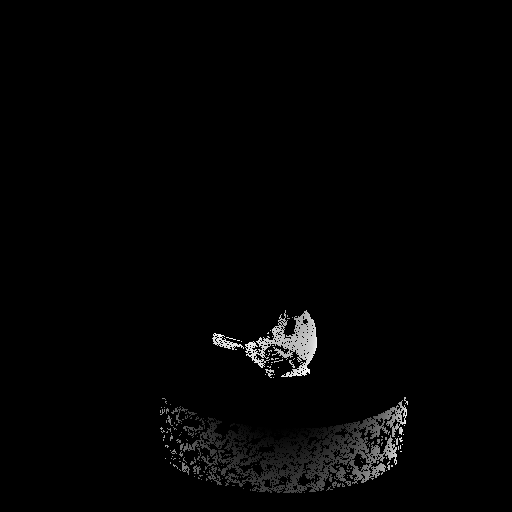
\includegraphics[width=.4\textwidth]{Figures/kinect-depth.png}
	\decoRule
	\caption{A captured depth map via infrared sensors. Pixels that far away represent by light colors, otherwise by dark colors. The black dots are the depths that failed to be detected.}
\label{fig:depth-map-with-noise}
\end{figure}


%% add noise image

\begin{figure}[th]
	\centering
	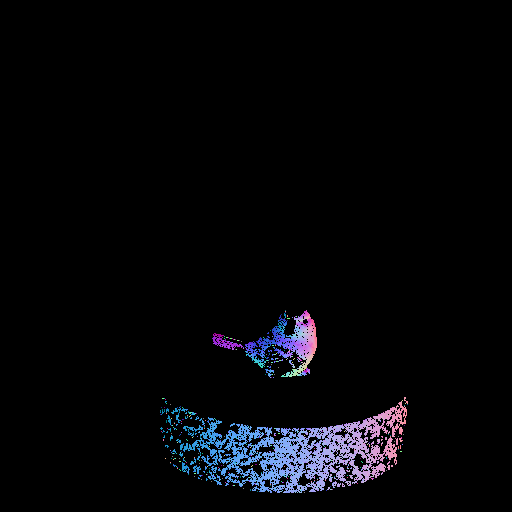
\includegraphics[width=.4\textwidth]{Figures/real-normal.png}
	\decoRule
	\caption{Semi-dense Normal Map calculated from depth map using a standard method}
\label{fig:standard-normal-inference}
\end{figure}


%%%%%%%%%%%%%%%%%% talk about the main work in this thesis  %%%%%%%%%%%%%%%%%%
\section{Main Works of this thesis}
In this thesis, we found a solution for the problems mentioned above and proposed a novel deep learning architecture for surface normal inference. A network named Albedo Gated Normal Inference Network(AlGaN) is proposed to infer normal given the corresponding depth map. The architecture of AlGaN involves a two-stage CNN. The first stage infers the normal map using point cloud as input. If the light source position and grayscale image can be provided further, the second stage infers the albedo altogether with the normals from the first stage. In addition, the loss function is based on least-square error and Lambertian reflection.

With the help of synthetic data in Unity, a dataset is created for CNN model training. It can provide accurate ground truth for training work, which real data is usually not provided. The results of this dataset show that our AlGaN model performs also well on real data captured by Infrared cameras. The trained Normal models achieve a remarkably better prediction accuracy at a low computational cost compared to the standard approaches for semi-dense point clouds. 